
\de{ĐỀ THI HỌC KỲ I NĂM HỌC 2022-2023}{Trường THPT Phạm Phú Thứ - Quảng Nam}
\begin{center}
	\textbf{PHẦN 1 - TRẮC NGHIỆM}
\end{center}
\Opensolutionfile{ans}[ans/ans]

%%=====Câu 1
\begin{ex}%[0D2Y2-1]%[Dự án đề kiểm tra HKI NH22-23-Thầy Hóa]%[THPT Phạm Phú Thứ]
Trong các cặp số sau, cặp nào \textbf{không} là nghiệm của hệ bất phương trình: $\heva{&x+y-2\leq 0\\&x-y+2>0}$?
\choice
{$(-1;-1)$}
{$(0;0)$}
{\True $(-1;1)$}
{$(1;1)$}
\loigiai{
Vì cặp số $(x;y)=(-1;1)$ không phải là nghiệm của bất phương trình $x-y+2>0$ nên cặp số $(-1;1)$ không phải là nghiệm của hệ bất phương trình đã cho.
}
\end{ex}

%%=====Câu 2
\begin{ex}%[0H2Y3-1]%[Dự án đề kiểm tra HKI NH22-23-Thầy Hóa]%[THPT Phạm Phú Thứ]
Gọi $G$ là trọng tâm của tam giác $ABC$ và điểm $M$ bất kỳ. Đẳng thức nào sau đây đúng?
\choice
{\True $\vec{MA}+\vec{MB}+\vec{MC}=3\vec{MG}$}
{$\vec{MA}+\vec{MB}+\vec{MC}=\vec{MG}$}
{$\vec{MA}+\vec{MB}+\vec{MC}=2\vec{MG}$}
{$\vec{MA}+\vec{MB}+\vec{MC}=4\vec{MG}$}
\loigiai{
\immini{
Theo tính chất trọng tâm, ta có
\[\vec{MA}+\vec{MB}+\vec{MC}=3\vec{MG}. \]
}{
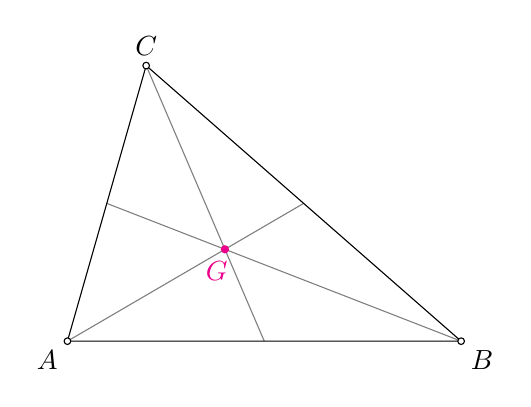
\begin{tikzpicture}
	\path
	(-1,0) coordinate (A) node[below left]{$A$}
	(4,0) coordinate (B) node[below right]{$B$}
	(0,3.5) coordinate (C) node[above]{$C$}
	(A)--(B) coordinate[pos=.5] (M)
	(B)--(C) coordinate[pos=.5] (N)
	(C)--(A) coordinate[pos=.5] (P);
	\draw[gray] (A)--(N) (B)--(P) (C)--(M);
	\draw (A)--(B)--(C)--cycle;
	% G là trọng tâm tam giác ABC
	\path (barycentric cs:A=1,B=1,C=1) coordinate (G);
	% vẽ điểm
	\fill[magenta] (G) circle(1.5pt) +(-110:.3) node{$G$};
	\foreach \p in {A,B,C}
	\draw[fill=white] (\p) circle(1.2pt);
\end{tikzpicture}
}
}
\end{ex}

%%=====Câu 3
\begin{ex}%[0H1B2-2]%[Dự án đề kiểm tra HKI NH22-23-Thầy Hóa]%[THPT Phạm Phú Thứ]
Cho tam giác $ABC$ biết $b=4$, $c=5$, $\widehat{A}=30^\circ$. Hãy tính diện tích $S$ của tam giác $ABC$.
\choice
{$S=10\sqrt{3}$}
{$S=10$}
{$S=20$}
{\True $S=5$}
\loigiai{
Ta có $S=\dfrac{1}{2}bc\sin A=\dfrac{1}{2}\cdot 4\cdot 5\cdot \sin 30^\circ=5$ (đơn vị diện tích).
}
\end{ex}

%%=====Câu 4
\begin{ex}%[0D1B2-2]%[Dự án đề kiểm tra HKI NH22-23-Thầy Hóa]%[THPT Phạm Phú Thứ]
Cho tập hợp $A=\{1;2;3;4\}$. Hỏi tập hợp $A$ có tất cả bao nhiêu tập con có một phần tử?
\choice
{$2$}
{$3$}
{$5$}
{\True $4$}
\loigiai{
Tập hợp $A$ có tất cả $4$ tập hợp con có một phần tử là
\[\{1\}; \{2\}; \{3\}; \{4\}. \]
}
\end{ex}

%%=====Câu 5
\begin{ex}%[0H2Y1-1]%[Dự án đề kiểm tra HKI NH22-23-Thầy Hóa]%[THPT Phạm Phú Thứ]
Cho các mệnh đề sau với các véc-tơ khác $\vec{0}$.
\begin{enumerate}[(I).]
	\item Hai véc-tơ cùng phương khi giá của chúng song song hoặc trùng nhau.
	\item Nếu hai véc-tơ ngược hướng thì chúng cùng phương.
	\item Nếu hai véc-tơ cùng phương thì chúng cùng hướng.
	\item Nếu hai véc-tơ bằng nhau thì chúng cùng độ dài.
\end{enumerate}
Có bao nhiêu mệnh đề đúng?
\choice
{$1$}
{$4$}
{\True $3$}
{$2$}
\loigiai{
Có tất cả $3$ mệnh đề đúng là (I), (II), (IV).
}
\end{ex}

%%=====Câu 6
\begin{ex}%[0H3B2-1]%[Dự án đề kiểm tra HKI NH22-23-Thầy Hóa]%[THPT Phạm Phú Thứ]
Cho $\vec{a}=(3;-2)$, $\vec{b}=(2;3)$, khi đó tích vô hướng $\vec{a}\cdot\vec{b}$ bằng
\choice
{$10$}
{$12$}
{\True $0$}
{$-12$}
\loigiai{
Ta có $\vec{a}\cdot\vec{b}=3\cdot 2+(-2)\cdot 3=0$.
}
\end{ex}

%%=====Câu 7
\begin{ex}%[0D1B3-2]%[Dự án đề kiểm tra HKI NH22-23-Thầy Hóa]%[THPT Phạm Phú Thứ]
Cho bảng số liệu về thống kê số điểm kiểm tra thường xuyên môn toán của $11$ học sinh có mẫu số liệu như sau:
\[5\quad 5\quad 7\quad 7\quad 6\quad 6\quad 7\quad 7\quad 8\quad 8\quad 9. \]
Hỏi số trung vị $M_e$ của mẫu số liệu trên?
\choice
{$M_e=5$}
{$M_e=8$}
{\True $M_e=7$}
{$M_e=6$}
\loigiai{
Mẫu số liệu được sắp xếp theo thứ tự tăng dần như sau
\[5\quad 5\quad 6\quad 6\quad 7\quad 7\quad 7\quad 7\quad 8\quad 8\quad 9. \]
Vì mẫu số liệu có $11$ giá trị nên số trung vị ở vị trí số $6$.\\
Vậy số trung vị của mẫu số liệu là $M_e=7$.
}
\end{ex}

%%=====Câu 8
\begin{ex}%[0D1Y1-1]%[Dự án đề kiểm tra HKI NH22-23-Thầy Hóa]%[THPT Phạm Phú Thứ]
Câu nào là mệnh đề?
\choice
{Không được sử dụng tài liệu khi kiểm tra}
{Hôm nay là thứ mấy?}
{\True Điện Trung là một xã trong vùng Gò Nổi}
{Bạn làm bài có tốt không?}
\loigiai{
Khẳng định ``Điện Trung là một xã trong vùng Gò Nổi'' là mệnh đề.
}
\end{ex}

%%=====Câu 9
\begin{ex}%[0H3Y1-3]%[Dự án đề kiểm tra HKI NH22-23-Thầy Hóa]%[THPT Phạm Phú Thứ]
Trong mặt phẳng tọa độ $Oxy$, cho $\vec{u}=3\vec{i}-2\vec{j}$. Tìm tọa độ của $\vec{u}$.
\choice
{$\vec{u}=(3;2)$}
{$\vec{u}=(-2;-3)$}
{$\vec{u}=(-2;3)$}
{\True $\vec{u}=(3;-2)$}
\loigiai{
Tọa độ của $\vec{u}$ là $(3;-2)$.
}
\end{ex}

%%=====Câu 10
\begin{ex}%[0H1Y1-2]%[Dự án đề kiểm tra HKI NH22-23-Thầy Hóa]%[THPT Phạm Phú Thứ]
Mệnh đề nào sau đây đúng?
\choice
{$\sin\left(180^\circ-x\right)=-\sin x$}
{\True $\sin\left(180^\circ-x\right)=\sin x$}
{$\tan\left(180^\circ-x\right)=\tan x$}
{$\cos\left(180^\circ-x\right)=\cos x$}
\loigiai{
Ta có $\sin\left(180^\circ-x\right)=\sin x$.
}
\end{ex}

%%=====Câu 11
\begin{ex}%[0D2Y1-1]%[Dự án đề kiểm tra HKI NH22-23-Thầy Hóa]%[THPT Phạm Phú Thứ]
Cặp số nào là một nghiệm của bất phương trình $x+2y-3>0$?
\choice
{$(-1;1)$}
{$(1;1)$}
{$(0;0)$}
{\True $(2;1)$}
\loigiai{
\begin{itemize}
	\item Ta có $-1+2\cdot 1-3>0$ sai nên cặp số $(-1;1)$ không là nghiệm của bất phương trình $x+2y-3>0$.
	\item Ta có $1+2\cdot 1-3>0$ sai nên cặp số $(1;1)$ không là nghiệm của bất phương trình $x+2y-3>0$.
	\item Ta có $0+2\cdot 0-3>0$ sai nên cặp số $(0;0)$ không là nghiệm của bất phương trình $x+2y-3>0$.
	\item Ta có $2+2\cdot 1-3>0$ đúng nên cặp số $(2;1)$ là nghiệm của bất phương trình $x+2y-3>0$.
\end{itemize}
}
\end{ex}

%%=====Câu 12
\begin{ex}%[0H2B2-3]%[Dự án đề kiểm tra HKI NH22-23-Thầy Hóa]%[THPT Phạm Phú Thứ]
Cho ba điểm $A$, $B$, $C$ bất kỳ. Mệnh đề nào sau đây \textbf{sai}?
\choice
{$\vec{AB}+\vec{BC}=\vec{AC}$}
{\True $\vec{AB}-\vec{AC}=\vec{BC}$}
{$\vec{AB}=\vec{AC}+\vec{CB}$}
{$\vec{BA}+\vec{AB}=\vec{0}$}
\loigiai{
\begin{itemize}
	\item Khẳng định $\vec{AB}+\vec{BC}=\vec{AC}$ là đúng (quy tắc cộng).
	\item Khẳng định $\vec{AB}-\vec{AC}=\vec{BC}$ sai vì $\vec{AB}-\vec{AC}=\vec{CB}$.
	\item Khẳng định $\vec{AB}=\vec{AC}+\vec{CB}$ là đúng (quy tắc cộng).
	\item Khẳng định $\vec{BA}+\vec{AB}=\vec{0}$ đúng (quy tắc cộng).
\end{itemize}
}
\end{ex}



\Closesolutionfile{ans}
\begin{center}
	\textbf{ĐÁP ÁN}
	\inputansbox{10}{ans/ans}	
\end{center}
\begin{center}
	\textbf{PHẦN 2 - TỰ LUẬN}
\end{center}

\begin{bt}%[0D1Y3-4]%[Dự án đề kiểm tra HKII NH22-23 - Thành Đức Trung]%[Sở Bắc Giang]
Cho hai tập hợp $A=(-3;2)$ và $B=[-1;4]$\\
Thực hiện phép toán trên tập hợp sau $A\cap B$; $A\cup B$.
\loigiai
{
Ta có $A\cap B=[-1;2)$ và $A \cup B=(-3;4]$.
}
\end{bt}

%%%% Câu 2 - Tự luận
\begin{bt}%[0H2B2-6]%[Dự án đề kiểm tra HKII NH22-23 - Thành Đức Trung]%[Sở Bắc Giang]
Hai người cùng kéo một khúc gỗ trên con suối với hai lực $\overrightarrow{F_1}$, $\overrightarrow{F_2}$ có độ lớn $\left|\overrightarrow{F_1}\right|=\left|\overrightarrow{F_2}\right|=100$N và góc tạo bởi hai lực $\overrightarrow{F_1}$, $\overrightarrow{F_2}$ là $60^\circ$. Hãy tính độ lớn của tổng hợp lực $\overrightarrow{F_1}$, $\overrightarrow{F_2}$. (hình vẽ tham khảo)
\begin{center}
\includegraphics[scale=0.5]{images/hk1-2022-2023-pham-thu-thu-quang-nam-cau-2}
\end{center}
\loigiai
{
\immini
{
Tổng hợp lực là đường chéo hình thoi
$$\overrightarrow{F_1}+\overrightarrow{F_2}=\overrightarrow{AB}+\overrightarrow{AC}=\overrightarrow{AD} \Rightarrow \left|\overrightarrow{F_1}+\overrightarrow{F_2}\right|=AD.$$
Ta có tam giác $ABC$ đều cạnh $100$, suy ra $AI=\dfrac{100\sqrt{3}}{2}$. \\
Mà $AD=2AI \Rightarrow AD=100\sqrt{3}$. \\
Vậy tổng hợp lực $\overrightarrow{F_1}$, $\overrightarrow{F_2}$ có độ lớn là $100\sqrt{3}$.
}
{
\begin{tikzpicture}[scale=0.7, font=\footnotesize, line join=round, line cap=round, >=stealth]
\draw(0,-3)--(0,3);
\draw[->](-4,0)--(4,0);
\draw[->](-4,0)--(0,3);
\draw[->](0,3)--(4,0);
\draw[->](-4,0)--(0,-3);
\draw[->](0,-3)--(4,0);
\path
(0,0)node[above left]{$I$}
(-4,0)node[left]{$A$}
(0,3)node[above]{$B$}
(0,-3)node[below]{$C$}
(4,0)node[right]{$D$}
;
\end{tikzpicture}
}
}
\end{bt}

%%%% Câu 3 - Tự luận
\begin{bt}%[0H2B3-5]%[Dự án đề kiểm tra HKII NH22-23 - Thành Đức Trung]%[Sở Bắc Giang]
Cho tam giác $ABC$ gọi $M$ là điểm thuộc đoạn $BC$ sao cho $MB=\dfrac{1}{3}MC$. Hãy phân tích $\overrightarrow{AM}$ theo véc-tơ $\overrightarrow{AB}$ và $\overrightarrow{AC}$.
\loigiai
{
\immini
{
Ta có
$$\begin{aligned}
& \ \overrightarrow{AM}=\overrightarrow{AB}+\overrightarrow{BM} \\
\Leftrightarrow & \ \overrightarrow{AM}=\overrightarrow{AB}+\dfrac{1}{3}\overrightarrow{BC} \\
\Leftrightarrow & \ \overrightarrow{AM}=\overrightarrow{AB}+\dfrac{1}{3}\left(\overrightarrow{AC}-\overrightarrow{AB}\right) \\
\Leftrightarrow & \ \overrightarrow{AM}=\dfrac{2}{3}\overrightarrow{AB}+\dfrac{1}{3}\overrightarrow{AC}.
\end{aligned}$$
}
{
\begin{tikzpicture}[scale=0.7, font=\footnotesize, line join=round, line cap=round, >=stealth]
\path
(0,0)coordinate(B)node[below]{$B$}
(2,0)coordinate(M)node[below]{$M$}
(8,0)coordinate(C)node[below]{$C$}
(2,4)coordinate(A)node[above]{$A$}
;
\draw(A)--(B)--(C)--(A)--(M);
\end{tikzpicture}
}
}
\end{bt}

%%%% Câu 4 - Tự luận
\begin{bt}%[0H3Y2-2]%[Dự án đề kiểm tra HKII NH22-23 - Thành Đức Trung]%[Sở Bắc Giang]
Cho hai véc-tơ $\overrightarrow{a}=(3;1)$, $\overrightarrow{b}=(2;4)$. Tính góc giữa hai véc-tơ $\overrightarrow{a}$ và $\overrightarrow{b}$.
\loigiai
{
Ta có $\cos \left(\overrightarrow{a},\overrightarrow{b}\right)=\dfrac{\overrightarrow{a}\cdot\overrightarrow{b}}{\left|\overrightarrow{a}\right|\cdot\left|\overrightarrow{b}\right|}=\dfrac{3\cdot2+1\cdot4}{\sqrt{3^2+1^2}\cdot\sqrt{2^2+4^2}}=\dfrac {\sqrt 2}{2} \Rightarrow \left(\overrightarrow{a},\overrightarrow{b}\right)=45^{\circ}$. \\
Vậy góc giữa hai véc-tơ $\overrightarrow{a}$ và $\overrightarrow{b}$ là $45^{\circ}$.
}
\end{bt}

%%%% Câu 5 - Tự luận
\begin{bt}%[0H3B1-4]%[Dự án đề kiểm tra HKII NH22-23 - Thành Đức Trung]%[Sở Bắc Giang]
Cho tam giác $ABC$ với $A(-1;4)$, $B(-2;1)$ và $C(2;1)$. Tìm tọa độ điểm $D$ để tứ giác $ABCD$ là hình bình hành.
\loigiai
{
Ta có $\overrightarrow{BC}=(4;0)$. \\
Gọi $D(x;y)$, suy ra $\overrightarrow{AD}=(x+1;y-4)$. \\
Để $ABCD$ là hình bình hành thì $\overrightarrow{AD}=\overrightarrow{BC} \Leftrightarrow \heva{ & x+1=4 \\ & y-4=0} \Leftrightarrow \heva{ & x=3 \\ & y=4.}$ \\
Vậy $D(3;4)$.
}
\end{bt}

%%%% Câu 6 - Tự luận
\begin{bt}%[0H2K4-1]%[Dự án đề kiểm tra HKII NH22-23 - Thành Đức Trung]%[Sở Bắc Giang]
Cho tam giác $ABC$. Gọi $M$ là trung điểm của $BC$, $H$ là trực tâm tam giác $ABC$ chứng minh rằng $\overrightarrow{MH}\cdot\overrightarrow{MA}=\dfrac{1}{4}BC^2$.
\loigiai
{
\immini
{
Ta có $\heva{ & \overrightarrow{AM}=\dfrac{1}{2}\left(\overrightarrow{AB}+\overrightarrow{AC}\right) \Rightarrow \overrightarrow{MA}=-\dfrac{1}{2}\left(\overrightarrow{AB}+\overrightarrow{AC}\right) \\ & \overrightarrow{HM}=\dfrac{1}{2}\left(\overrightarrow{HB}+\overrightarrow{HC}\right) \Rightarrow \overrightarrow{MH}=-\dfrac{1}{2}\left(\overrightarrow{HB}+\overrightarrow{HC}\right).}$ \\
Suy ra
$$\begin{aligned}
\overrightarrow{MH}\cdot\overrightarrow{MA}
&=\dfrac{1}{4}\left(\overrightarrow{AB}+\overrightarrow{AC}\right)\cdot\left(\overrightarrow{HB}+\overrightarrow{HC}\right) \\
&=\dfrac{1}{4}\left(\overrightarrow{AB}\cdot\overrightarrow{HB}+\overrightarrow{AB}\cdot\overrightarrow{HC}+\overrightarrow{AC}\cdot\overrightarrow{HB}+\overrightarrow{AC}\cdot\overrightarrow{HC}\right).
\end{aligned}$$
}
{
\begin{tikzpicture}[scale=1, font=\footnotesize, line join=round, line cap=round, >=stealth]
\path
(1,3)coordinate(A)
(0,0)coordinate(B)
(4,0)coordinate(C)
($(B)!(A)!(C)$)coordinate(A_0)
($(A)!(B)!(C)$)coordinate(B_0)
($(B)!0.5!(C)$)coordinate(M)
(intersection of A--A_0 and B--B_0)coordinate(H)
;
\draw(A)--(B)--(C)--(A)--(M)--(H)--(B) (H)--(C);
\foreach \p/\q in {A/90, B/-90, C/-90, M/-90, H/90} \fill[black] (\p) circle (1pt) ($(\p)+(\q:2.5mm)$) node{$\p$};
\end{tikzpicture}
}
\noindent
Ta có $\heva{ & \overrightarrow{AB}\perp\overrightarrow{HC} \Rightarrow \overrightarrow{AB}\cdot\overrightarrow{HC}=0 \\ & \overrightarrow{AC}\perp\overrightarrow{HB} \Rightarrow \overrightarrow{AC}\cdot\overrightarrow{HB}=0.}$ \\
Do đó
$$\begin{aligned}
\overrightarrow{MH}\cdot\overrightarrow{MA}
&=\dfrac{1}{4}\left(\overrightarrow{AB}\cdot\overrightarrow{HB}+\overrightarrow{AC}\cdot\overrightarrow{HC}\right) \\
&=\dfrac{1}{4}\left(\overrightarrow{AB}\cdot\left(\overrightarrow{HC}+\overrightarrow{CB}\right)+\overrightarrow{AC}\cdot\left(\overrightarrow{HB}+\overrightarrow{BC}\right)\right) \\
&=\dfrac{1}{4}\left(\overrightarrow{AB}\cdot\overrightarrow{HC}+\overrightarrow{AB}\overrightarrow{CB}+\overrightarrow{AC}\cdot\overrightarrow{HB}+\overrightarrow{AC}\cdot\overrightarrow{BC}\right) \\
&=\dfrac{1}{4}\left(0-\overrightarrow{AB}\cdot\overrightarrow{BC}+0+\overrightarrow{AC}\cdot\overrightarrow{BC}\right)=\dfrac{1}{4}\overrightarrow{BC}\cdot\left(\overrightarrow{AC}-\overrightarrow{AB}\right) \\
&=\dfrac{1}{4}\overrightarrow{BC}\cdot\overrightarrow{BC}=\dfrac{1}{4}\overrightarrow{BC}^2 \\
&=\dfrac{1}{4}BC^2.
\end{aligned}$$
}
\end{bt}